\section{Indoor Ranges}
\begin{definition}{Indoor Ranges}
  Indoor antenna ranges are enclosed facilites that mimic or simulate a free-space condition.
\end{definition}

\subsection{Electrically shielded chambers}
\begin{itemize}
  \item High power testing
  \item Complience with radio frequency interference regulations
  \item Test of classified equipment
\end{itemize}

\subsection{Microwave Absorbers}
\begin{itemize}
        \item Pyramidal Absorbers
        \begin{itemize}
          \item Most common
          \item Pyramid length: $\geq 1 \lambda$\\
                (max absorber size $\approx \SI{2.44}{m} \implies \lambda_{\text{min}} \approx \SI{123}{MHz}$)
          \item Better attenuation at higher frequencies
            \item Significant reflections for oblique angles
        \end{itemize}
        \item Wedge Absorbers (common in tapered chambers)
  \item Flat Absorbers
        \begin{itemize}
          \item In chamber edges
          \item Inferior to pyramidal absorbers
        \end{itemize}
        \item Walkable Absorbers
\end{itemize}

\subsection{Anechoic chambers}
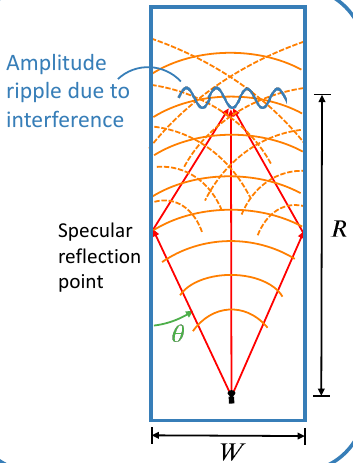
\includegraphics[height=5cm]{content/at_meas/pictures/rectangular_anechoic_chamber}
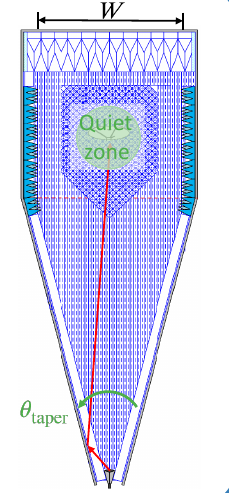
\includegraphics[height=5cm]{content/at_meas/pictures/tapered_anechoic_chamber}
\begin{itemize}
  \item $W \geq \frac{R}{\sqrt{3}}$ for rect.
        \item $\theta_{\text{taper}} \leq 30^{\circ}$, $W \geq 3$ quiet zone sizes for tapered
\end{itemize}

\section{Compact Ranges}
\begin{definition}{Compact Range}
  Generate a plane wave illumination of an AUT over a specified test zone (``quiet zone'') in a relatively short distance.
\end{definition}
Different design types
\begin{itemize}
  \item Transformation by lens
  \item Plane Wave Generator (antenna array)
  \item Transformation by reflector
  \item Surface accuracy of $0.007\lambda$; half for dual reflectors
\end{itemize}
